
Explain the specific challenges in the strip detector that are parameterized and modeled
in our case.

\subsubsection{DCDC converter}

The DCDC converter (FEAST) supplies a low-voltage (1.5~V) current to the ABC130 and HCC front-end
chips on the module.
The efficiency of the FEAST depends on its temperature as well as the output (load) current
load delivered to the front-end chips. To correctly model the FEAST efficiency, experimental
measurements are performed to characterize the dependence and fitted with a functional form.

To measure the FEAST efficiency, the FEAST power board was glued to an aluminum cold plate, cooled
with CO$_2$, an powered with the nominal working input and output voltages (11~V input, 1.5~V output).
The temperature of the FEAST is measured with an NTC thermistor and PTAT sensor residing on the FEAST,
for a range of load currents up to the maximum design current of 4A\footnote
{
FEAST data spreadsheet: \url{http://project-dcdc.web.cern.ch/project-dcdc/public/Documents/FEASTMod_Datasheet.pdf}.
Cite?
}.

The data is then fit with a function with sufficient parameters to ensure reasonable agreement; the
choice of functional form has no physical interpretation. Figure~\ref{fig:feast_eff} depicts the
FEAST efficiency data and the parameterized fit used in the model.

\begin{figure}[ht]
\centering
\subfloat[] {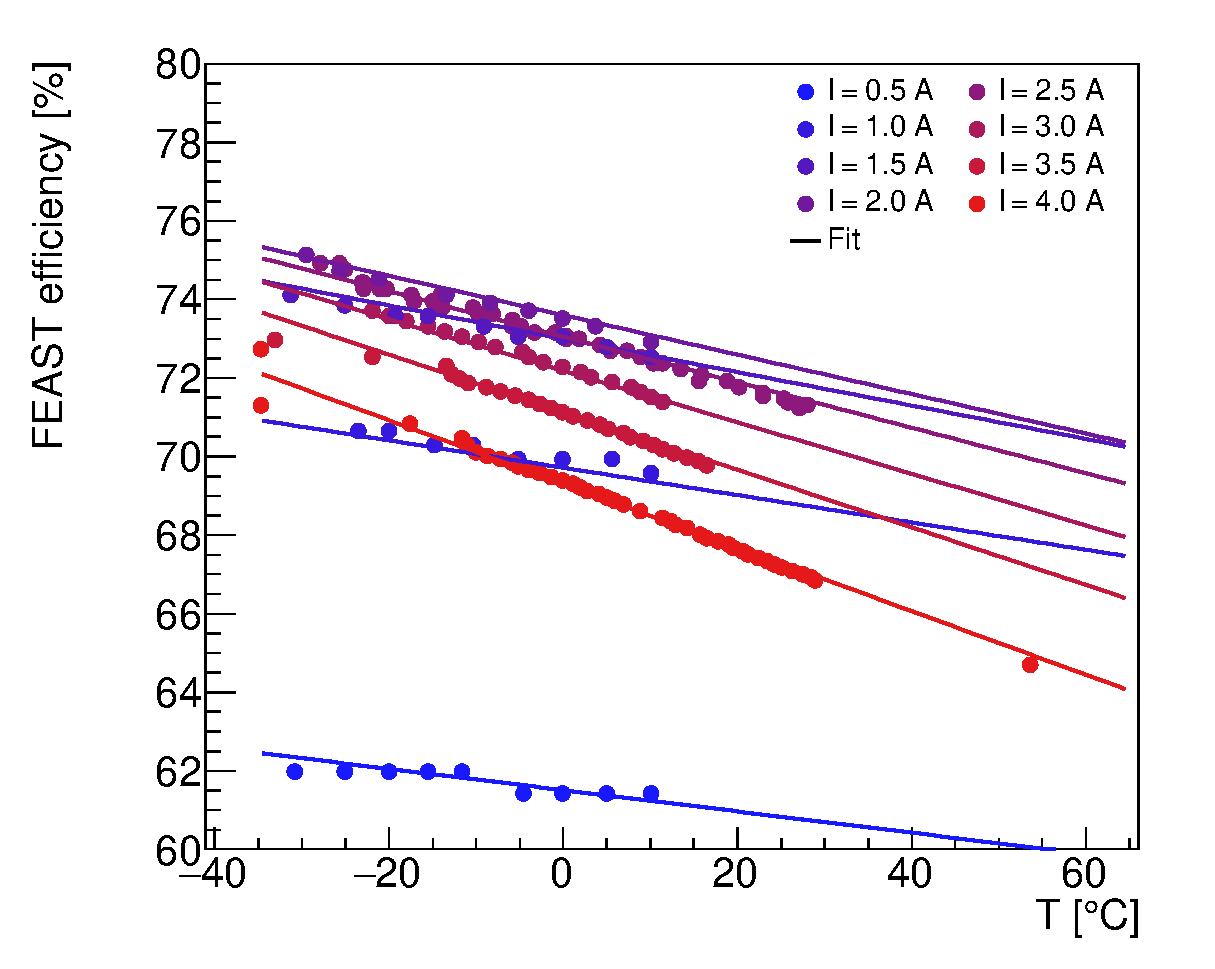
\includegraphics[width=0.49\linewidth]{figures/FeastEfficiency_isoCurrent.eps}}
\subfloat[] {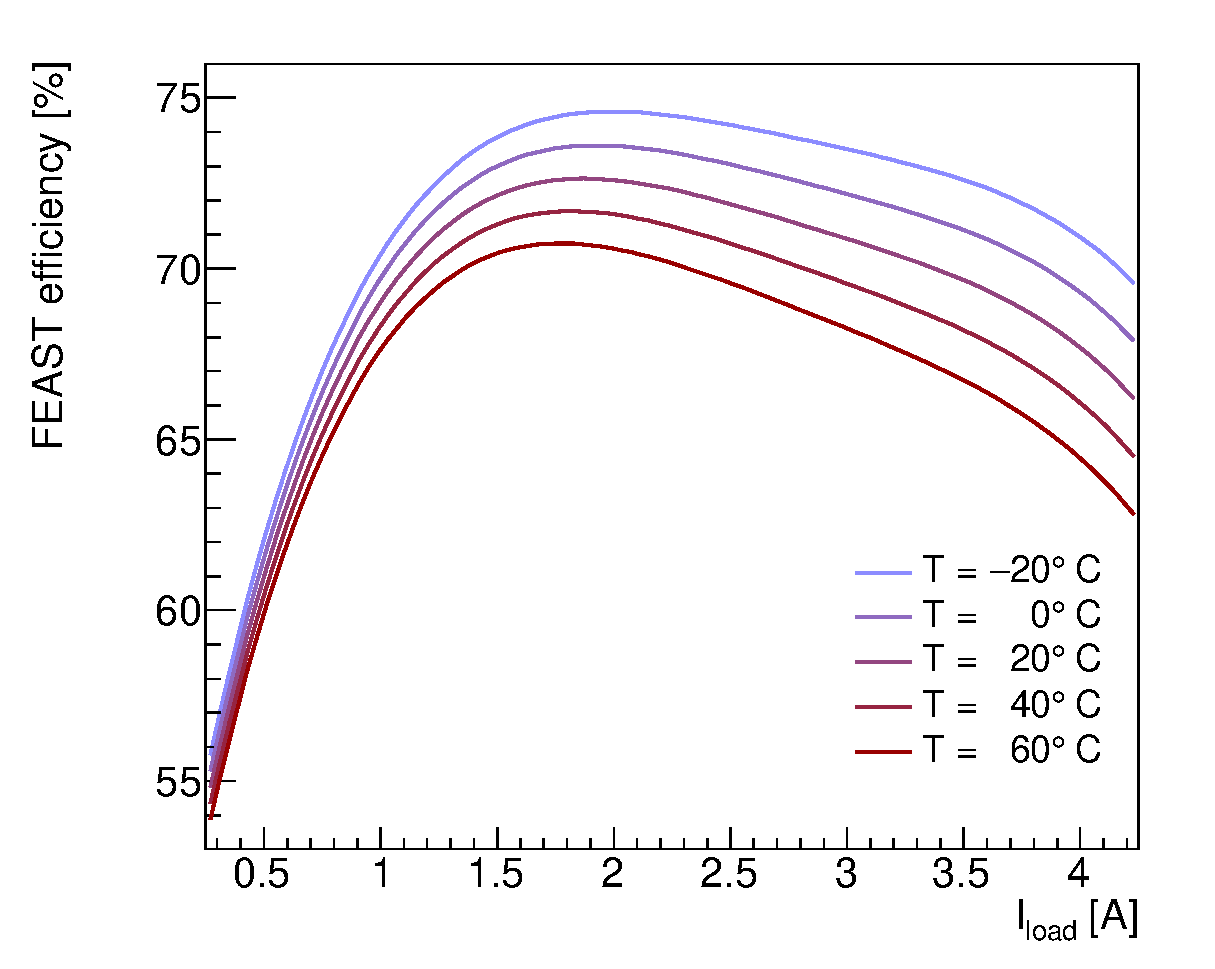
\includegraphics[width=0.49\linewidth]{figures/FeastEfficiency.eps}}
\caption{The FEAST efficiency model based on experimental data. (a) The experimental data points
characterizing the FEAST efficiency are plotted as dots and color coded for load current. The data is
compared to the analytic fit, evaluated in curves of equal current. (b) The same analytic fit,
presented as a function of current load for curves of equal temperature.
}
\label{fig:feast_eff}
\end{figure}


\subsubsection{Digital current increase of chips using 130~nm CMOS technology}
\label{sec:tid_explanation}

The ABC and HCC chips, designed using IBM 130 nm CMOS8RF technology, are known to suffer from an
increase in digital current when subjected to a high-radiation environment
\cite{Collaboration:2017mtb}. This phenomenon, known as the ``TID bump,'' is well-studied
\cite{1589217,FACCIO20081000} and has a characteristic shape whereby the effect reaches a maximum
over a period of time and then gradually diminishes (see Fig.~\ref{tid_bump}).

In an effort to characterize the nature of the TID bump in the ABC and HCC chips empirically,
many irradiation campaigns have been conducted using a variety of radiation sources, testing
the effect at different temperatures and dose rates.
The data collected from these studies was used to develop a model of the TID bump
that estimates the digital current increase given the total ionizing dose, the dose rate,
and the operating temperature of the chip. This parameterization, which is depicted in
Fig~\ref{tid_bump}, is used as an input to the thermoelectric model in order to correctly model the
ABC and HCC currents. The TID bump is assumed to fully apply to the HCC digital current, and apply to
69\% of the ABC digital current (according to our understanding of its digital circuitry).

\begin{figure}[ht]
\centering
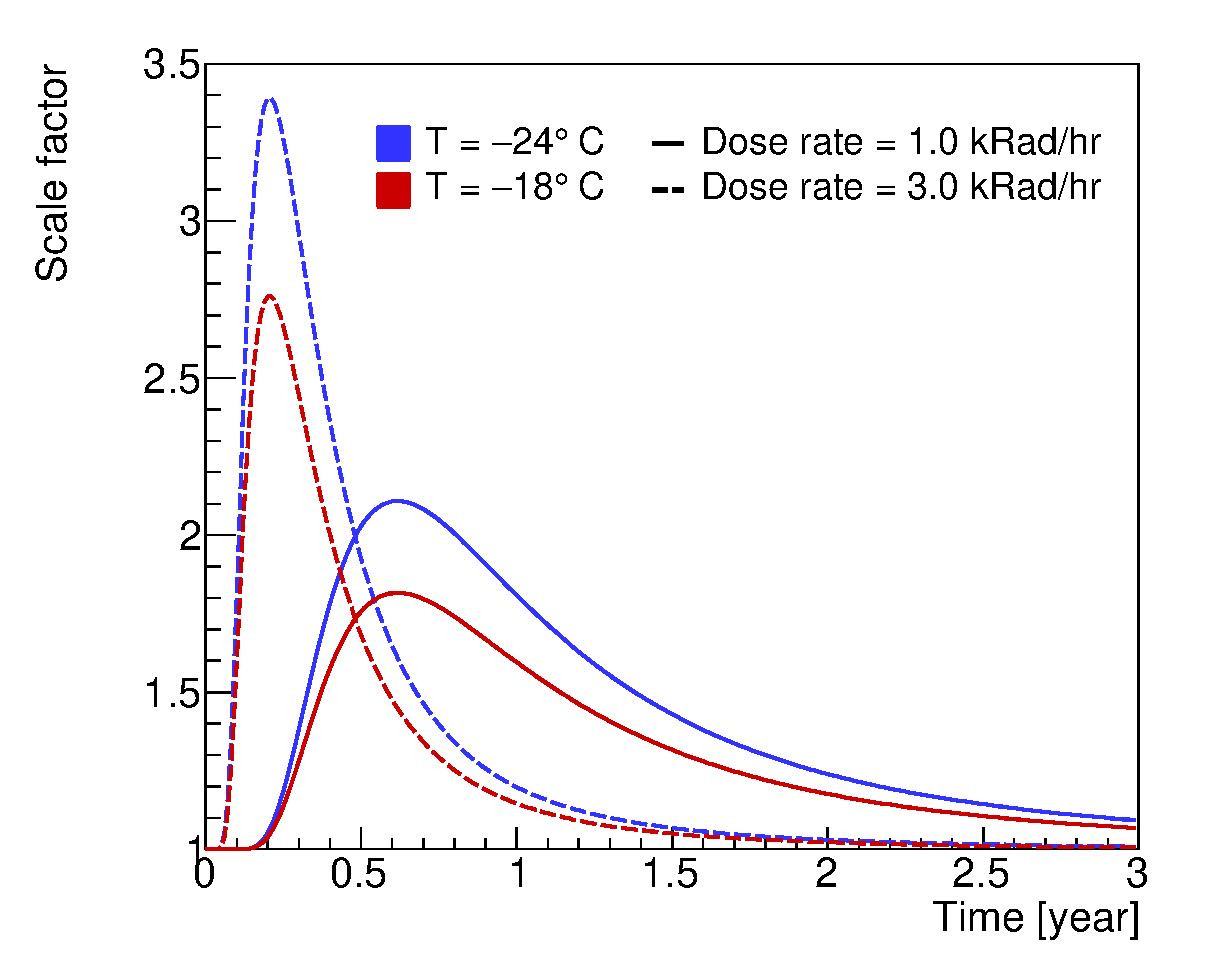
\includegraphics[width=0.5\linewidth]{figures/AbcTidBumpVersionRatesAndTemps_Nominal.eps}
\caption{Parameterization of the impact of the total ionizing dose
on the magnitude of the front-end chip digital current (the TID bump), presented as a function of time.
The current is multiplied by a scale factor that is modeled as a function of total ionizing dose,
dose rate, and temperature, based on experimental data.
}
\label{tid_bump}
\end{figure}

The TID bump displays certain key features, which are reflected in the parameterization:
first, the effect is larger at colder temperatures and higher dose rates. This means it can be
mitigated by operating the chips at higher temperature (note that the dose rate is fixed by the LHC conditions).
Second, the figure also illustrates how chips receiving different dose rates will reach their maximum
digital current increase at different times. This feature is particularly important when modeling the
total power consumed by the barrel and endcap systems. In both systems, the dose rate varies significantly
depending on the position of the module in the detector. The effect means that the maximum system
power will be smaller than the sum of the maximum power of each module, as each chip reaches
its maximum at a different point in time.

\subsubsection{Modeling flux and total ionizing dose in endcap modules}

Covered already in the introduction?

